\chapter{Solution}
\label{cha:solution}

\sloppy

This chapter will present the \texttt{xmlet} solution, its different components and how they interact between them. Generating a Java \ac{API} based on a \ac{XSD} file includes two distinct tasks:

\begin{enumerate}
\item Parsing the information from the \ac{XSD} file;
\item Generating the \ac{API} based on the resulting information of the previous task.
\end{enumerate}

\noindent
Those tasks are encompassed by two different projects, \hyperref[sec:xsdparser]{XsdParser} and \hyperref[sec:xsdasm]{XsdAsm}. In this case the XsdAsm has a dependency to XsdParser.

\section{XsdParser} % (fold)
\label{sec:xsdparser}

XsdParser is a library that parses a \ac{XSD} file into a list of Java objects. Each different \ac{XSD} tag has a corresponding Java class and the  attributes of a given \ac{XSD} type are represented as fields in Java. All these classes derive from the same abstract class, \texttt{XsdAbstractElement}. All Java representations of the \ac{XSD} elements follow the schema definition for \ac{XSD} elements, referred in Section \ref{sec:xsd}. For example, the \texttt{xsd:annotation} tag only allows \texttt{xsd:appinfo} and \texttt{xsd:documentation} as children nodes, and can also have an attribute named \texttt{id}, therefore XsdParser has the following class as shown in Listing \ref{lst:xsdannotationexample}.

\bigskip

\lstset{language=java, morekeywords={XsdAppInfo, XsdDocumentation, ArrayList, List, XsdIdentifierElements, Document, parse, getFirstChild, getChildNodes, NodeList, DocumentBuilderFactory, DocumentBuilder, newInstance, newDocumentBuilder}}

\begin{minipage}{\linewidth}
\begin{lstlisting}[caption={XsdAnnotation class (Simplified)}, label={lst:xsdannotationexample}]
public class XsdAnnotation extends XsdIdentifierElements {

    //The id field is inherited from XsdIdentifierElements.
    private List<XsdAppInfo> appInfoList = new ArrayList<>();
    private List<XsdDocumentation> documentations = new ArrayList<>();
\end{lstlisting}
\end{minipage}

\subsection{Parsing Strategy}
\label{sec:parsingstrategy}

The first step of this library is handling the \ac{XSD} file. The Java language has no built in library that parses \ac{XSD} files, so we needed to look for other options. The main libraries found that address this problem were \ac{DOM} and \ac{SAX}. After evaluating the pros and cons of those libraries the choice ended up being \ac{DOM}. This choice was based mostly on the fact that \ac{SAX} is an event driven parser and \ac{DOM} is a tree based parser, which is more adequate for the present issue. \ac{DOM} is a library that maps \ac{HTML}, \ac{XHTML} and \ac{XML} files into a tree structure composed by multiple elements, also named nodes. This is exactly what XsdParser requires to obtain all the information from the \ac{XSD} files, which is described in \ac{XML}. 

\noindent
This means that XsdParser uses \ac{DOM} to parse the \ac{XSD} file into a node list, performing a single read on the \ac{XSD} file, avoiding multiple reads which is less efficient (Listing \ref{lst:nodelist}). 

\bigskip

\lstset{language=java, morekeywords={Document, parse, getFirstChild, getChildNodes, NodeList, DocumentBuilderFactory, DocumentBuilder, newInstance, newDocumentBuilder}}

\begin{minipage}{\linewidth}
\begin{lstlisting}[caption={DOM Document Parsing}, label={lst:nodelist}]
DocumentBuilderFactory dbFactory= DocumentBuilderFactory.newInstance();
DocumentBuilder dBuilder = dbFactory.newDocumentBuilder();
//Parses the XSD file
Document doc = dBuilder.parse(xsdFile);
//Obtains the XSD file node list
NodeList nodes = doc.getFirstChild().getChildNodes();
\end{lstlisting}
\end{minipage}

\newpage

\noindent
Then parsing the continues by iterating this list (i.e. nodes) and obtaining the name of the element represented by that node, e.g. \texttt{xsd:element} or \texttt{xsd:complexType}. The name of the element will be needed to perform a lookup search to find the corresponding parsing function (Listing \ref{lst:nodeparsingprocess}). 

\medskip

\lstset{language=Java, morekeywords={stream, filter, map, forEach, apply, add, getNodeType, getNodeName, get, Node}}
\begin{minipage}{\linewidth}
\begin{lstlisting}[caption={XsdParser Node Parsing Process},captionpos=b,label={lst:nodeparsingprocess}]
stream(nodes)
    .filter(node -> 
        node.getNodeType() == Node.ELEMENT_NODE && 
        parseMappers.get(node.getNodeName()) != null)
    .map(node -> 
        parseMappers.get(node.getNodeName())
                        .apply(node))
    .forEach(elements::add);
\end{lstlisting}
\end{minipage}

\noindent
From that moment on each element obtains all its attribute information directly from its node object (Listing \ref{lst:xsdattributeparsing}). 

\medskip

\lstset{language=Java, morekeywords={getOrDefault, NamedNodeMap, Map, String, getAttributes, convertNodeMap}}
\begin{minipage}{\linewidth}
\begin{lstlisting}[caption={XsdAttribute Information Extraction (Simplified)},captionpos=b,label={lst:xsdattributeparsing}]
public class XsdAttribute extends XsdReferenceElement {
    private XsdAttribute(Map<String, String> elementFieldsMapParam) {
        setFields(elementFieldsMapParam);
    }

    @Override
    public void setFields(Map<String, String> elementFieldsMapParam) {
        super.setFields(elementFieldsMapParam);

        this.fixed = elementFieldsMap.getOrDefault(FIXED_TAG, fixed);
        this.type = elementFieldsMap.getOrDefault(TYPE_TAG, type);
        this.form = elementFieldsMap.getOrDefault(FORM_TAG, form);
        this.use = elementFieldsMap.getOrDefault(USE_TAG, "optional");
        this.defaultElement = elementFieldsMap.getOrDefault(DEFAULT_ELEMENT_TAG, defaultElement);
    }
    
    public static ReferenceBase parse(Node node) {
        NamedNodeMap nodeAttributes = node.getAttributes();
        Map<String, String> attrMap = convertNodeMap(nodeAttributes);        
        XsdAttribute attribute = new XsdAttribute(attrMap);    
    
        return xsdParseSkeleton(node, attribute);
    }
}
\end{lstlisting}
\end{minipage}

\noindent
Regarding the other elements that may be contained in a given node they are all similarly parsed. The \texttt{xsdParseSkeleton} function existing in the \texttt{XsdAbstractElement} class (Listing \ref{lst:skeletonfunction}) will iterate in all the children of a given node, invoke the respective \texttt{parse} function of each one and then notify the parent element, using the Visitor pattern, so that the parent element can perform the changes needed based on the element received.

\bigskip

\lstset{language=Java, morekeywords={Node, XsdAbstractElement, getFirstChild, getNodeType, getNodeName, String, Function, getParseMappers, get, apply, getElement, accept, getVisitor, getNextSibling, createFromXsd, ReferenceBase}}
\begin{minipage}{\linewidth}
\begin{lstlisting}[caption={XsdParseSkeleton Parsing Children From a Node},captionpos=b,label={lst:skeletonfunction}]
static ReferenceBase xsdParseSkeleton(Node node, XsdAbstractElement element){
    Node child = node.getFirstChild();

    //Iterates in all children from the received Node object, node.
    while (child != null) {   
        //Only parses element nodes, ignoring comments and text nodes.
        if (child.getNodeType() == Node.ELEMENT_NODE) { 
            //Obtains the name of the node, e.g. xsd:element.
            String nodeName = child.getNodeName();

            //Searches on a mapper for a parsing functions 
            //for the respective type.
            Function<Node, ReferenceBase> parserFunction = XsdParser.getParseMappers().get(nodeName);

            //Applies the parsing functions, if any, and notifies 
            //the parent objects Visitor to the newly created object.
            if (parserFunction != null){
                parserFunction.apply(child)
                                   .getElement()
                                   .accept(element.getVisitor());
            }
        }

        //Moves on to the next sibling.
        child = child.getNextSibling();
    }

    //Wraps the element in a ReferenceBase object, 
    //which will be explained further ahead.
    return ReferenceBase.createFromXsd(element);
}
\end{lstlisting}
\end{minipage}

\newpage

\noindent
Based on the explanation provided above, we will give a more detailed description about the parsing process made by XsdParser using a concrete example with the \ac{XSD} code present in Listing \ref{lst:parsingexample}.

\bigskip

\lstset{
	language=XML,
	morekeywords={xsd:element, xsd:complexType, id}
}

\begin{minipage}{\linewidth}
\begin{lstlisting}[caption={Parsing Concrete Example},captionpos=b,label={lst:parsingexample}]
<xsd:element>
		<xsd:complexType id="complexId">
				<!-- (...) -->
		</xsd:complexType>
</xsd:element>
\end{lstlisting}
\end{minipage}


Step 1 - DOM parsing:

\noindent
The parsing starts with the \ac{DOM} library parsing the code (Listing \ref{lst:parsingexample}), which returns a node list (i.e. nodes) containing only one node, the \texttt{xsd:element} node. Using the \texttt{xsd:element} string the \texttt{XsdElement parse} function will be obtained from an existent string to function mapper (i.e. parseMappers). 

Step 2 - XsdElement Attribute Parsing:

\noindent
The \texttt{XsdElement parse} function receives the \texttt{Node} object and extracts all the attribute information (similar to the example presented in Listing \ref{lst:xsdattributeparsing}), which in this case is empty since the element has no attributes. 

Step 3 - XsdElement Children:

\noindent
To parse the \texttt{XsdElement} children the \texttt{XsdAbstractElement xsdParseSkeleton} function is called (Listing \ref{lst:skeletonfunction}) and starts to iterate the \texttt{xsd:element} node children, which is a node list containing a single element, the \texttt{xsd:complexType} node. 

Step 4 - XsdComplexType Attribute Parsing:

\noindent
The parsing of the \texttt{xsd:complexType} node is similar to \texttt{xsd:element}, it extracts the attribute information from its respective node, in this case it will obtain a value from the node attribute named \texttt{id} and assigning it to the \texttt{id} field of the \texttt{XsdCompleType} object (similar to the example presented in Listing \ref{lst:xsdattributeparsing}). 

Step 5 - XsdElement Visitor Notification:

\noindent
After parsing the \texttt{xsd:compleType} node the previously created \texttt{XsdElement} object is notified. This notification informs the \texttt{XsdElement} object that it contains the newly created \texttt{XsdCompleType} object using the Visitor pattern. The \texttt{XsdElement} should then act accordingly based on the type of the object received as his children, since different types of objects should be treated differently. 

\noindent
This whole behaviour is shared by all the classes that represent a \ac{XSD} element. The Visitor pattern is a very important tool in the parsing process since it allows each element to define a different behaviour for each element received as children. This is also useful to implement the schema rules, since it can be used to define empty methods to reject any children that a given element type shouldn't contain as per definition on the schema specification. The same happens to the attributes present in the parsed \ac{DOM} nodes, each XsdParser object only extracts the attributes defined in the \ac{XSD} schema specification, ignoring other attributes present.

\subsection{Reference solving}
\label{sec:refsolving}

After the parsing process described previously, there is still an issue to solve regarding the existing references in the \ac{XSD} schema definition. In \ac{XSD} files the usage of the ref attribute is frequent to avoid repetition of \ac{XML} code. This generates two main problems when handling reference solving, the first one being existing elements with ref attributes referencing non existent elements and the other being the replacement of the reference object by the referenced object when present. In order to effectively help resolve the referencing problem some wrapper classes were added. These wrapper classes contain the wrapped element and serve as a classifier for the wrapped element. The existing wrapper classes are as follow:

\begin{itemize}  
	\item UnsolvedElement - Wrapper class to each element that was not found in the file.
	\item ConcreteElement - Wrapper class to each element that is present in the file.
	\item NamedConcreteElement - Wrapper class to each element that is present in the file and has a name attribute present.
	\item ReferenceBase - A common interface between UnsolvedReference and ConcreteElement.
\end{itemize}

\noindent
Having these wrappers on the elements allow for a detailed filtering, which is helpful in the reference solving process. That process starts by obtaining all the \texttt{NamedConcreteElement} objects since they may or may not be referenced by an existing \texttt{UnsolvedReference} object. The second step is to obtain all the \texttt{UnsolvedReference} objects and iterate them to perform a lookup search on the \texttt{NamedConcreteElement} objects obtained previously. This is achieved by comparing the value present in the \texttt{UnsolvedReference ref} attribute with the \texttt{NamedConcreteElement name} attribute. If a match is found then XsdParser performs a copy of the object wrapped by the \texttt{NamedConcreteElement} and replaces the element wrapped in the \texttt{UnsolvedReference} object that served as a placeholder. A concrete example of how this process works is in Listing \ref{lst:refsolvingexample}.

\bigskip

\lstset{
	language=XML,
	morekeywords={encoding, xsd:schema, xmlns, xmlns:xsd, xsd:group, xsd:choice, id, name,  ref}
}

\begin{minipage}{\linewidth}
\begin{lstlisting}[caption={Reference Solving Example},captionpos=b,label={lst:refsolvingexample}]
<?xml version='1.0' encoding='utf-8' ?>
<xsd:schema xmlns='http://schemas.microsoft.com/intellisense/html-5' xmlns:xsd='http://www.w3.org/2001/XMLSchema'>
	
    <!-- NamedConcreteType wrapping a XsdGroup -->
    <xsd:group id="replacement" name="flowContent">
				<!-- (...) -->
    </xsd:group>
	
    <!-- ConcreteElement wrapping a XsdChoice -->
    <xsd:choice>
        <!-- UnsolvedReference wrapping a XsdGroup -->
        <xsd:group id="toBeReplaced" ref="flowContent"/>
    </xsd:choice>
</xsd:schema>
\end{lstlisting}
\end{minipage}

\noindent
In this short example we have a \texttt{XsdChoice} element that contains a \texttt{XsdGroup} element with a reference attribute. When replacing the \texttt{UnsolvedReference} objects the \texttt{XsdGroup} with the \texttt{ref} attribute is going to be replaced by a copy of the already parsed \texttt{XsdGroup} with the \texttt{name} attribute. This is achieved by accessing the parent of the element, in this case accessing the parent of the \texttt{XsdGroup} with the \texttt{ref} attribute, in order to remove the element identified by "toBeReplaced" and adding the element identified by "replacement".

\noindent
Having created these classes it is expected that at the end of a successful file parsing only \texttt{ConcreteElement} and/or \texttt{NamedConcreteElement} objects remain. In case there are any remainder \texttt{UnsolvedReference} objects the programmer can query the parser, using the function \texttt{getUnsolvedReferencesForFile(String filePath)}, to discover which elements are missing and where were they used. The programmer can then correct the missing elements by adding them to the \ac{XSD} file and repeat the parsing process or just acknowledge that those elements are missing. 

\section{XsdAsm} % (fold)
\label{sec:xsdasm}

XsdAsm is a library dedicated to generate a fluent Java \ac{API} based on a \ac{XSD} file. It uses the previously introduced XsdParser library to parse the \ac{XSD} file contents into a list of Java elements that XsdAsm will use to obtain the information needed to generate the correspondent classes. To generate classes this library also uses the ASM\footnote{\href{http://asm.ow2.org/}{ASM Website}} library, which is a library that provides a Java interface to bytecode manipulation, which provide method for creating classes, methods, etc. There were other alternatives to the ASM library but most of them are simply libraries that were built on top of ASM to simplify its usage. It supports the creation of Java classes up until Java 9 and is still maintained, the most recent version, 6.1, was release in 11 march of 2018. ASM also has some tools to help the new programmers understand how the library works. These tools help the programmers to learn faster how the code generation works and allow to increase the complexity of the generated code.

\subsection{Supporting Infrastructure}
\label{sec:supportinginfrastructure}

To support the foundations of the \ac{XSD} language an infrastructure is created in every \ac{API} generated by this project. This infrastructure is composed by a common set of classes. This supporting infrastructure is divided into three different groups of classes:

Element classes:

\begin{itemize}  
	\item Element - An interface that serves as a base to every parsed \ac{XSD} element.
	\item AbstractElement - An abstract class from where all the \ac{XSD} element derive. This class implements most of the methods present on the Element interface.
\end{itemize}

Attribute classes:

\begin{itemize}  
	\item Attribute - An interface that serves as a base to every parsed \ac{XSD} attribute.
	\item BaseAttribute - A class that implements the Attribute interface and adds restriction verification to all the deriving classes. All the attributes that have restrictions should derive from this class.
\end{itemize}

Visitor classes:

\begin{itemize}
	\item ElementVisitor - An interface that defines methods for all the generated elements that can be visited with the Visitor pattern. All the methods have a default implementation that point to a single method. This behaviour aims to reduce the amount of code needed to create concrete implementations of  Visitors.
\end{itemize}

\noindent
Taking in consideration those classes, a very simplistic \ac{API} could be represented with the class diagram (Figure \ref{img:infrastructure}). In this example we have an element, \texttt{Html}, that extends \texttt{AbstractElement} and an attribute, \texttt{AttrManifestString}, that extends \texttt{BaseAttribute}. 

\begin{figure}[h]
	\centering
	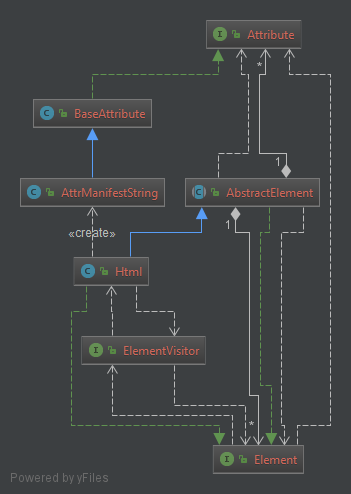
\includegraphics[width=0.6\textwidth]{infrastructure}
	\caption{API - Supporting Infrastructure}
	\label{img:infrastructure}
\end{figure}

\subsection{Code Generation Strategy}
\label{sec:codegenerationstrategy}

\noindent
To understand how most of this project works a \ac{XSD} example (Listing \ref{lst:codegenerationexample}) and a detailed explanation is provided. In this example there will be some simplifications making it easier to understand how the library works internally.

\bigskip

\lstset{
	language=XML,
	morekeywords={xs:element, name, xs:complexType, xs:choice, ref, xs:attributeGroup, xs:attribute, type}
}

\begin{minipage}{\linewidth}
\begin{lstlisting}[caption={Code Generation XSD Example},captionpos=b, ,label={lst:codegenerationexample}]
<xs:element name="html">
    
    <xs:attributeGroup name="commonAttributeGroup">
        <xs:attribute name="someAttribute" type="xs:string">
    </xs:attributeGroup>

    <xs:complexType>
        <xs:choice>
            <xs:element ref="body"/>
            <xs:element ref="head"/>
        </xs:choice>
        <xs:attributeGroup ref="commonAttributeGroup" />
        <xs:attribute name="manifest" type="xs:string" />
    </xs:complexType>
    
</xs:element>
\end{lstlisting}
\end{minipage}

\noindent
With this example there is a multitude of classes that need to be created, apart from the always present supporting infrastructure presented in Section \ref{sec:supportinginfrastructure}. 

\begin{itemize}
	\item Html Element - A class that represents the \texttt{Html} element (Listing \ref{lst:htmlclass}), deriving from \texttt{AbstractElement}.
	\item Body and Head Methods - Both methods present in the \texttt{Html} class (Listing \ref{lst:htmlclass}) that add \texttt{Body} (Listing \ref{lst:bodyclass}) and \texttt{Head} (Listing \ref{lst:headclass}) instances to \texttt{Html} children list.
	\item Manifest Method - A method present in \texttt{Html} class (Listing \ref{lst:htmlclass}) that adds an instance of the \texttt{Manifest} attribute (Listing \ref{lst:manifestattributeclass}) to the \texttt{Html} attribute list.
\end{itemize}

\newpage

\lstset{language=Java, morekeywords={AbstractElement, CommonAttributeGroup, Body, addChild, Head, String, AttrManifest, addAttr}}

\begin{lstlisting}[caption={Html Element Class},captionpos=b,label={lst:htmlclass}]
public class Html extends AbstractElement implements CommonAttributeGroup {
    public Html() { }
    
    public Html attrManifest(String attrManifest) {
        this.addAttr(new AttrManifest(attrManifest));
    }
    
    public Body body() { this.addChild(new Body()); }
        
    public Head head() { this.addChild(new Head()); }
}
\end{lstlisting}

\begin{itemize}
	\item Body and Head classes - Classes for both \texttt{Body} (Listing \ref{lst:bodyclass}) and \texttt{Head} (Listing \ref{lst:headclass}) elements, similar to the generated \texttt{Html} class (Listing \ref{lst:htmlclass}). The class contents will be dependent on the contents present in the concrete \texttt{xsd:element} nodes.
\end{itemize}

\bigskip

\begin{minipage}{\linewidth}
\begin{lstlisting}[caption={Body Element Class},captionpos=b,label={lst:bodyclass}]
public class Body extends AbstractElement {
    //Similar to Html, based on the contents of the respective
    //xsd:element node.
}
\end{lstlisting}
\end{minipage}

\bigskip

\begin{minipage}{\linewidth}
\begin{lstlisting}[caption={Head Element Class},captionpos=b,label={lst:headclass}]
public class Head extends AbstractElement {
    //Similar to Html, based on the contents of the respective 
    //xsd:element node.
}
\end{lstlisting}
\end{minipage}

\begin{itemize}
	\item Manifest Attribute - A class that represents the \texttt{Manifest} attribute  (Listing \ref{lst:manifestattributeclass}), deriving from \texttt{BaseAttribute}.
\end{itemize}

\bigskip

\lstset{language=Java, morekeywords={String, BaseAttribute}}

\begin{minipage}{\linewidth}
\begin{lstlisting}[caption={Manifest Attribute Class},captionpos=b,label={lst:manifestattributeclass}]
public class AttrManifestString extends BaseAttribute<String> {
    public AttrManifestString(String attrValue) {
        super(attrValue);
    }
}
\end{lstlisting}
\end{minipage}

\begin{itemize}
	\item CommonAttributeGroup Interface - An interface with default methods that add the group attributes to the concrete element (Listing \ref{lst:commonattributegroup}).
\end{itemize}

\bigskip

\lstset{language=Java, morekeywords={addAttr, Html, Element, String, SomeAttribute}}

\begin{minipage}{\linewidth}
\begin{lstlisting}[caption={CommonAttributeGroup Interface},captionpos=b,label={lst:commonattributegroup}]
public interface CommonAttributeGroup extends Element {
    default Html attrSomeAttribute(String attributeValue) {
        this.addAttr(new SomeAttribute(attributeValue));
        return this;
    }
}
\end{lstlisting}
\end{minipage}

\noindent
As we can see from the previous example this solution focus on how the code is organized instead of making complex code. All the methods present in the generated classes have very low complexity, mainly adding information to the element children and attribute list. To reduce repeated code many interfaces with default methods are created so different classes can implement them and reuse the code. The complexity of the generated code is mostly present in the \texttt{AbstractElement} class, which implements most of the \texttt{Element} interface methods. Another very important aspect of the generated classes is the extensive use of type arguments which allows the \ac{API} to navigate in the element tree while maintaining type information which is essential to guarantee the specific language restrictions.

\subsection{Restriction Validation}
\label{sec:restrictionvalidation}

In the description of any given \ac{XSD} file there are many restrictions in the way the elements are contained in each other and which attributes are allowed. To reflect those restrictions to Java language there are two alternatives, validation in runtime or in compile time. This library tries to validate most of the restrictions in compile time, as shown above by the way classes are created. But some restrictions can't be validated in compile time, an example of this is the following restriction (Listing \ref{lst:restrictionexample}):

\bigskip

\lstset{
	language=XML,
	morekeywords={xs:schema, xs:element, name, xs:complexType, xs:attribute, name, type, xs:simpleType, xs:restriction, xs:maxLength, xs:minLength, value, xs:list, itemType}
}

\begin{minipage}{\linewidth}
\begin{lstlisting}[caption={Restrictions Example},captionpos=b,label={lst:restrictionexample}]
<xs:schema>
    <xs:element name="testElement">
        <xs:complexType>
            <xs:attribute name="intList" type="valuelist"/>
        </xs:complexType>
    </xs:element>
    
    <xs:simpleType name="valuelist">
        <xs:restriction>
            <xs:maxLength value="5"/>
            <xs:minLength value="1"/>
        </xs:restriction>
        <xs:list itemType="xsd:int"/>
    </xs:simpleType>
</xs:schema>
\end{lstlisting}
\end{minipage}

\noindent
In this example (Listing \ref{lst:restrictionexample}) we have an element (i.e. testElement) that has an attribute called \texttt{intList}. This attribute has some restrictions, it is represented by a \texttt{xs:list}, the list elements have the \texttt{xsd:int} type and its element count should be between 1 and 5. Transporting this example to the Java language will result in the following class (Listing \ref{lst:attributeclassexample}):

\lstset{language=Java, morekeywords={BaseAttribute, List, Integer}}

\begin{minipage}{\linewidth}
\begin{lstlisting}[caption={Attribute Class Example},captionpos=b,label={lst:attributeclassexample}]
public class AttrIntList extends BaseAttribute<List> {
    public AttrIntList(List<Integer> list) {
        super(list);
    }
}
\end{lstlisting}
\end{minipage}

\noindent
But with this solution the \texttt{xs:maxLength} and \texttt{xs:minLength} values are ignored. To solve this problem the existing restrictions in any given attribute are hardcoded in the class static constructor, which stores the restrictions in a static \texttt{Map} object as showed in Listing \ref{lst:attrhardcodedrestrictions}.

\bigskip

\lstset{language=Java, morekeywords={ArrayList, HashMap, String, Object, valueOf, add, put}}

\begin{minipage}{\linewidth}
\begin{lstlisting}[caption={Attribute Static Constructor Restrictions},captionpos=b,label={lst:attrhardcodedrestrictions}]
static {
    restrictions = new ArrayList<Map<String, Object>();
    HashMap<String, Object> restriction = new HashMap<>();
    restriction.put("MaxLength", Integer.valueOf(5));
    restriction.put("MinLength", Integer.valueOf(1));
    restrictions.add(restriction);
}
\end{lstlisting}
\end{minipage}

\noindent
By using this strategy the restrictions can be validated whenever an instance of a concrete attribute is created. To enforce the restrictions present in the \texttt{Map} object the \texttt{BaseAttribute} constructor (Listing \ref{lst:baseattributeconstructor}) will pass those values to a class, \texttt{RestrictionValidator}, which validates all the different types of restrictions, in this case \texttt{xs:maxlength} and \texttt{xs:minlength}. Each different restriction has its validation method (i.e. \texttt{validateMaxLength} and \texttt{validateMinLength} at Listing \ref{lst:restrictionvalidator} lines 6 and 11, respectively) which will throw an exception if the value (i.e. val) to validate does not match the restriction. By using this strategy the \ac{API} ensures that any successful usage follows the rules previously defined by the schema.

\bigskip

\lstset{language=Java, morekeywords={BaseAttribute, List, Integer, Map, String, Object, ArrayList, forEach, RestrictionsValidator, validate, Float, Double, Short, RestrictionValidator}}

\begin{minipage}{\linewidth}
\begin{lstlisting}[caption={BaseAttribute Rule Validation Restrictions},label={lst:baseattributeconstructor}]
public class BaseAttribute<T> implements Attribute<T> {
    static List<Map<String, Object>> restrictions = new ArrayList();

    public BaseAttribute(T var1, String var2) {
        // ...
        restrictions.forEach(this::validateRestrictions);
    }
    
    private void validateRestrictions(Map<String, Object> restriction){
        Object value = this.getValue();
        
        if (value instanceof String) {
            RestrictionValidator.validate(restriction, (String)value);
        }

        if (value instanceof Integer || value instanceof Short || 
             value instanceof Float || value instanceof Double) {
            RestrictionValidator.validate(restriction, (Double)value);
        }

        if (value instanceof List) {
            RestrictionValidator.validate(restriction, (List)value);
        }
    }
}
\end{lstlisting}
\end{minipage}

\bigskip

\lstset{language=Java, morekeywords={Map, String, Object, Double, getOrDefault, RestrictionViolationException, size, List}}

\begin{minipage}{\linewidth}
\begin{lstlisting}[caption={Restriction Validator Class (Simplified)},label={lst:restrictionvalidator}]
public class RestrictionValidator {
    static void validate(Map<String, Object> restMap, List val) {
        validateMinLength(restMap.getOrDefault("MinLength", -1), val);
        validateMaxLength(restMap.getOrDefault("MaxLength", -1), val);
    }
    private static void validateMaxLength(int maxLength, List list) {
        if (maxLength != -1 && list.size() > maxLength) {
            throw new RestrictionViolationException("Violation of maxLength restriction.");
        }
    }
    private static void validateMinLength(int minLength, List list) {
        if (minLength != -1 && list.size() < minLength) {
            throw new RestrictionViolationException("Violation of minLength restriction.");
        }
    }
}
\end{lstlisting}
\end{minipage}

\subsubsection{Enumerations}
\label{sec:enumarations}

Regarding restrictions there is one that can be enforced at compile time, the \texttt{xs:enumeration}. To obtain that validation at compile time the XsdAsm library generates \texttt{Enum} classes that contain all the values indicated in the \texttt{xs:enumeration} tags. In the following example (Listing \ref{lst:enumxsddefinition}) we have an attribute with three possible values, command, checkbox and radio.

\bigskip

\lstset{
	language=XML,
	morekeywords={xs:attribute, xs:simpleType, xs:restriction, base, xs:enumeration, value, name}
}

\begin{minipage}{\linewidth}
\begin{lstlisting}[caption={Enumeration XSD Definition},label={lst:enumxsddefinition}]
<xs:attribute name="type">
    <xs:simpleType>
        <xs:restriction base="xsd:string">
            <xs:enumeration value="command" />
            <xs:enumeration value="checkbox" />
            <xs:enumeration value="radio" />
        </xs:restriction>
    </xs:simpleType>
</xs:attribute>
\end{lstlisting}
\end{minipage}

\newpage

\noindent
This results in the creation of an \texttt{Enum}, \texttt{EnumTypeCommand} (Listing \ref{lst:enumclass}). The attribute class will then receive an instance of \texttt{EnumTypeCommand}, ensuring that only allowed values are used (Listing \ref{lst:enumusage}).

\bigskip

\lstset{language=Java, morekeywords={enum, String, valueOf}}

\begin{minipage}{\linewidth}
\begin{lstlisting}[caption={Enumeration Class},label={lst:enumclass}]
public enum EnumTypeCommand {
    COMMAND(String.valueOf("command")), 
    CHECKBOX(String.valueOf("checkbox")),
    RADIO(String.valueOf("radio"))
}
\end{lstlisting}
\end{minipage}

\lstset{language=Java, morekeywords={getValue, EnumTypeCommand, String, BaseAttribute}}

\begin{minipage}{\linewidth}
\begin{lstlisting}[caption={Attribute Receiving An Enumeration},label={lst:enumusage}]
public class AttrTypeEnumTypeCommand extends BaseAttribute<String> {
    public AttrTypeEnumTypeCommand(EnumTypeCommand attrValue) {
        super(attrValue.getValue());
    }
}
\end{lstlisting}
\end{minipage}

\subsection{Element Binding}
\label{sec:elementbinding}

\noindent
To support repetitive tasks over an element the \texttt{Element} and \texttt{AbstractElement} classes were modified to support binders. This allows programmers to define, for example, templates for a given element. An example is presented in Listing \ref{lst:binderusage} using the \ac{HTML}5 \ac{API}.

\bigskip

\lstset{language=Java, morekeywords={Html, Body, body, Table, .table, tr, th, text, binder, forEach, td, table, List, String}}

\begin{minipage}{\linewidth}
\begin{lstlisting}[caption={Binder Usage Example},label={lst:binderusage}]
public class BinderExample{
    public void bindExample(){
        Html<Html> root = new Html<>();
        Body<Html<Html>> body = root.body();
        
        Table<Body<Html<Html>>> table = body.table();
        table.tr().th().text("Title");
        table.<List<String>>binder((elem, list) ->
                        list.forEach(tdValue ->
                            elem.tr().td().text(tdValue)
                        )
                    );
        //Keep adding elements to the body of the document.
    }
}
\end{lstlisting}
\end{minipage}

\noindent
In this example we create a table and add a title in the first row as a title header (i.e. \texttt{th()}). In regard to the values present in the table instead of having them inserted right away it is possible delay that insertion by indicating what will the element do when the information is received. This is achieved by implementing a Visitor that supports binding. 

\noindent
In Listing \ref{lst:visitorbinding} we can observe how the Visitor would work. It maintains the default behaviour on the elements that aren't bound (i.e. else clause). In the case that the element is bound to a function this implementation will clone the element and apply a model (i.e. a List<String> object following the example of Listing \ref{lst:binderusage}) to the clone, effectively executing the function supplied in the previously called binder method (i.e. Listing \ref{lst:binderusage} line 8). This function call will generate new children on the cloned table element which will be iterated as if they belonged to the original element tree. This behaviour ensures that the original element tree isn't affected since all these changes are performed in a clone of the bound element, meaning that the template can be reused.

\bigskip

\lstset{language=Java, morekeywords={isBound, List, Element, cloneElem, bindTo, getChildren, forEach, accept}}

\begin{minipage}{\linewidth}
\begin{lstlisting}[caption={Visitor with binding support},label={lst:visitorbinding}]
public <T extends Element> void sharedVisit(Element<T, ?> element) {
    // ...
    
    if(element.isBound()) {
        List<Element> children = element.cloneElem()
                                        .bindTo(model)
                                        .getChildren();
        children.forEach( child -> child.accept(this));
    } else {
        element.getChildren().forEach(item -> item.accept(this));
    }
    
    // ...
}
\end{lstlisting}
\end{minipage}
        
\newpage

\section{Client} % (fold)
\label{sec:client}

To use and test both \hyperref[sec:xsdasm]{XsdAsm} and \hyperref[sec:xsdparser]{XsdParser} we need to implement a client for XsdAsm. Two different clients were implemented, one using the \ac{HTML}5 specification and another using the specification for Android visual layouts. In this section we are going to explore how the \ac{HTML}5 \ac{API} is generated using the XsdAsm library and how to use the resulting \ac{API}.

\subsection{HtmlApi}

To generate the \ac{HTML}5 \ac{API} we need to obtain its \ac{XSD} file. After that there are two options, the first one is to create a Java project that invokes the XsdAsm main method directly by passing the path of the specification file and the desired \ac{API} name (Listing \ref{lst:directapicreation}).

\bigskip

\lstset{language=Java, morekeywords={XsdAsmMain, String}}

\begin{minipage}{\linewidth}
\begin{lstlisting}[caption={API creation},label={lst:directapicreation}]
void generateApi(String filePath, String apiName){
    XsdAsmMain.main(new String[] {filePath, apiName} );    
}
\end{lstlisting}
\end{minipage}

\noindent
The second option is using the Maven\footnote{\href{https://maven.apache.org/}{Maven}} build lifecycle\footnote{\href{https://maven.apache.org/guides/introduction/introduction-to-the-lifecycle.html\#Build_Lifecycle_Basics}{Maven Build Lifecycle}} to make that same invocation by adding an extra execution to the \ac{POM} file (Listing \ref{lst:mavencreation}) to execute a batch file that invokes the XsdAsm main method (Listing \ref{lst:creationbat}). 

\bigskip

\lstset{language=XML, morekeywords={plugin, artifactId, groupId, executions, execution, id, phase, goals, goal, configuration, executable, basedir}}

\begin{minipage}{\linewidth}
\begin{lstlisting}[caption={Maven API compile classes plugin},label={lst:mavencreation}]
<plugin>
    <artifactId>exec-maven-plugin</artifactId>
    <groupId>org.codehaus.mojo</groupId>
    <version>1.6.0</version>
    <executions>
        <execution>
            <id>create_classes1</id>
            <phase>validate</phase>
            <goals>
                <goal>exec</goal>
            </goals>
            <configuration>
                <executable>
                    ${basedir}/create_class_binaries.bat
                </executable>
            </configuration>
        </execution>
    </executions>
</plugin>
\end{lstlisting}
\end{minipage}

\lstset{language=bash, morekeywords={exist, not, call, mvn, java, mkdir, rmdir}}

\begin{minipage}{\linewidth}
\begin{lstlisting}[caption={Maven API creation batch file (create\_class\_binaries.bat)},label={lst:creationbat}]
if exist "./src/main/java" rmdir "./src/main/java" /s /q

if not exist "./target/classes/org/xmlet/htmlapi" 
    mkdir "./target/classes/org/xmlet/htmlapi"

call 
    mvn exec:java -D"exec.mainClass"="org.xmlet.xsdasm.main.XsdAsmMain" 
    -D"exec.args"="./src/main/resources/html_5.xsd htmlapi"
\end{lstlisting}
\end{minipage}

\noindent
This client uses the Maven lifecycle option by adding an execution at the validate phase (Listing \ref{lst:mavencreation}, line 8) which invokes XsdAsm main method to create the \ac{API}. This invocation of XsdAsm creates all the classes in the target folder of the HtmlApi project. Following these steps would be enough to allow any other Maven project to add a dependency to the HtmlApi project and use its generated classes as if they were manually created. But this way the source files and Java documentation files are not created since XsdAsm only generates the class binaries. To tackle this issue we added another execution to the \ac{POM}. This execution uses the Fernflower\footnote{\href{https://mvnrepository.com/artifact/org.jboss.windup.decompiler/decompiler-fernflower/4.0.0.Final}{Fernflower Decompiler}} decompiler, the Java decompiler used by Intellij\footnote{\href{https://www.jetbrains.com/idea/}{Intellij IDE}} \ac{IDE}, to decompile the classes that were automatically generated (Listing \ref{lst:mavendecompilation}, \ref{lst:decompilationbat}). 

\bigskip

\lstset{language=XML, morekeywords={plugin, artifactId, groupId, executions, execution, id, phase, goals, goal, configuration, executable, basedir}}

\begin{minipage}{\linewidth}
\begin{lstlisting}[caption={Maven API decompile classes plugin},label={lst:mavendecompilation}]
<!-- Plugin Information -->
<execution>
    <id>decompile_classes</id>
    <phase>validate</phase>
    <goals>
        <goal>
            exec
        </goal>
    </goals>
    <configuration>
        <executable>
            ${basedir}/decompile_class_binaries.bat
        </executable>
    </configuration>
</execution>
\end{lstlisting}
\end{minipage}

\lstset{language=bash, morekeywords={exist, not, call, mvn, java, mkdir, rmdir}}

\begin{minipage}{\linewidth}
\begin{lstlisting}[caption={Maven API decompile batch file (decompile\_class\_binaries.bat)},label={lst:decompilationbat}]
if not exist "./src/main/java/org/xmlet/htmlapi" mkdir "./src/main/java/org/xmlet/htmlapi"

call 
    mvn exec:java 
    -D"exec.mainClass"="org.jetbrains.java.decompiler.main.decompiler.ConsoleDecompiler" 
    -D"exec.args"="-dgs=true ./target/classes/org/xmlet/htmlapi ./src/main/java/org/xmlet/htmlapi"

if exist "./target/classes/org" rmdir "./target/classes/org" /s /q
\end{lstlisting}
\end{minipage}

\noindent
By decompiling those classes we obtain the source code which allows us to delete the automatic generated classes and allow the Maven build process to perform the normal compiling process, which generates the Java documentation files and the class binaries, along with the source files obtained from the decompilation process. This process, apart from generating more information to the programmer that will use the \ac{API} in the future, also allows to find any problem with the generated code since it forces the compilation of all the classes previously generated.

\subsubsection{Using the HtmlApi}

After the previously described compilation process of the HtmlApi project we are ready to use the generated \ac{API}. To start using it the first step is to implement a custom Visitor class, which defines what to do when the created element tree is visited. A very simple example is presented in Listing \ref{lst:customvisitorexample} which writes the \ac{HTML} tags based on the name of the element visited and navigates in the element tree by accessing the children of the current element.

\bigskip

\lstset{language=Java, morekeywords={PrintStream, Element, T, ElementVisitor, getChildren, forEach, accept, out, printf, getAttributes, getName, getValue, print}}

\begin{minipage}{\linewidth}
\begin{lstlisting}[caption={Custom Visitor},label={lst:customvisitorexample}]
public class CustomVisitor<R> implements ElementVisitor<R> {

    private PrintStream printStream = System.out;

    public CustomVisitor(){ }

    public <T extends Element> void sharedVisit(Element<T, ?> element) {
        printStream.printf("<%s", element.getName());

        element.getAttributes()
               .forEach(attribute -> 
                   printStream.printf(" %s=\"%s\"", 
                       attribute.getName(), attribute.getValue()));

        printStream.print(">\n");

        element.getChildren().forEach(item -> item.accept(this));

        printStream.printf("</%s>\n", element.getName());
    }
}
\end{lstlisting}
\end{minipage}

\noindent
After creating the Visitor presented in Listing \ref{lst:customvisitorexample} we can start to create the element tree that we want convert to text using the \texttt{CustomVisitor}. To start we should create a \texttt{Html} object, since all the \ac{HTML} documents have it as a base element. Upon creating that root element we can start to add other elements or attributes that will appear as options based on the specification rules. To help with the navigation on the element tree a method was created to allow the navigation to the parent of any given element. This method is named \texttt{\textdegree}, a short method name to keep the code as clean as possible. In Listing \ref{lst:htmlapicodeexample} we can see a code example that uses a good amount of the \ac{API} features, including element creation and how they are added to the element tree, how to add attributes, attributes that receive enumerations as parameters and how to navigate in the element tree using the method \texttt{\textdegree}.

\bigskip

\lstset{language=Java, morekeywords={Html, head, meta, attrCharset, title, text, link, attrType, \textdegree, EnumTypeContentType, TEXT, CSS, attrHref, link, body, attrClass, div, header, section, div, img, attrId, attrSrc, aside, em, text, span, CustomVisitor, visit}}

\begin{minipage}{\linewidth}
\begin{lstlisting}[caption={HtmlApi Element Tree},label={lst:htmlapicodeexample}, literate={º}{\textdegree}1]
Html<Html> root = new Html<>();

root.head()
        .meta().attrCharset("UTF-8").º()
        .title()
            .text("Title").º()
        .link().attrType(EnumTypeContentType.TEXT_CSS)
                 .attrHref("/assets/images/favicon.png").º()
        .link().attrType(EnumTypeContentType.TEXT_CSS)
                 .attrHref("/assets/styles/main.css").º().º()
     .body().attrClass("clear")
        .div()
            .header()
                .section()
                    .div()
                        .img().attrId("brand")
                                .attrSrc("./assets/images/logo.png").º()
                        .aside()
                            .em()
                                .text("Advertisement")
                            .span()
                                .text("HtmlApi is great!");
                                    
CustomVisitor customVisitor = new CustomVisitor();
    
customVisitor.visit(root);
\end{lstlisting}
\end{minipage}

\noindent
With this element tree presented (Listing \ref{lst:htmlapicodeexample}) and the previously presented \texttt{CustomVisitor} (Listing \ref{lst:customvisitorexample}) we obtain the following result (Listing \ref{lst:htmlapiresult}). The indentation was added for readability purposes, since the \texttt{CustomVisitor} implementation in Listing \ref{lst:customvisitorexample} does not indent the resulting \ac{HTML}.

\bigskip

\lstset{language=html, morekeywords={header, section, aside}}

\begin{minipage}{\linewidth}
\begin{lstlisting}[caption={HtmlApi Visitor Result},label={lst:htmlapiresult}]
<html>
    <head>
        <meta charset="UTF-8">
        </meta>
        <title>
            Title
        </title>
        <link type="text/css" href="/assets/images/favicon.png">
        </link>
        <link type="text/css" href="/assets/styles/main.css">
        </link>
    </head>
    <body class="clear">
        <div>
            <header>
                <section>
                    <div>
                        <img id="brand" src="./assets/images/logo.png">
                        </img>
                        <aside>
                            <em>
                                Advertisement
                                <span>
                                    HtmlApi is great!
                                </span>
                            </em>
                        </aside>
                    </div>
                </section>
            </header>
        </div>
    </body>
</html>                          
\end{lstlisting}
\end{minipage}

\noindent
The \texttt{CustomVisitor} of Listing \ref{lst:htmlapiresult} is a very minimalist implementation since it does not indent the resulting \ac{HTML}, does not simplify elements with no children (i.e. the link/img elements) and other aspects that are particular to \ac{HTML} syntax. That is where the HtmlFlow library come in, it implements the particular aspects of the \ac{HTML} syntax in its Visitor implementation which deals with how and where the output is written. 